%   Filename    : chapter_2.tex 
\chapter{Review of Related Literature}
\label{sec:relatedlit}

Aquaculture is the fastest-growing industry in animal food production and has great potential as a sustainable solution to global food security, nutrition, and development \cite{fao2024}. Aquaculture is deeply integrated into the livelihoods of Filipinos, not only through fish cultivation but also through the production of other aquatic species, including mollusks, oysters, clams, scallops, and mussels \cite{breton2017sex}. Mollusks, particularly blood clams \Tegillarcagranosa, have economic and environmental significance. It has been a collective effort to maintain an ideal male-to-female ratio to avoid overharvesting and maintain the optimal ratio to preserve the population and production of the blood cockles. 
	
The members of the Arcidae Family, including \Tgranosa are important sources of food and livelihood. Cockle aquaculture meets rising demands, however, it faces significant challenges due to fluctuating seed supplies \cite{miranda2023}. To solve the problem, researchers exert a considerable amount of effort, developing a broader understanding of bivalves including their sex-determining mechanism due to their notable importance in terms of diversity, environmental benefits, and economic and market importance \cite{breton2017sex}. Despite the promising idea of identifying sex, there is limited research reported in terms of sexual dimorphism, making it harder to distinguish through its morphological and morphometric characteristics. 

By addressing the challenges in the sex identification of \Tgranosa, it would be able to address one problem at a time. Currently, no recent documented publications that integrate machine learning and computer vision in characterizing sexual dimorphism, reducing complexity, variability in sex determination, and differentiation mechanisms in bivalves, including \Tgranosa specifically.

\section{Background on \textit{\Tegillarcagranosa} and Their Importance}
\textit{\Tegillarcagranosa}(Linnaeus, 1758) is also known as blood cockles or blood clam. In the Philippines, it is commonly known as a Litob, a marine bivalve species from the family Arcidae. Litob is widely distributed in the world including Southeast Asia. They can be found in the intertidal mudflats adjacent to the mangrove forest \cite{srisunont2020}.

\begin{figure}[!htbp]
	\centering
	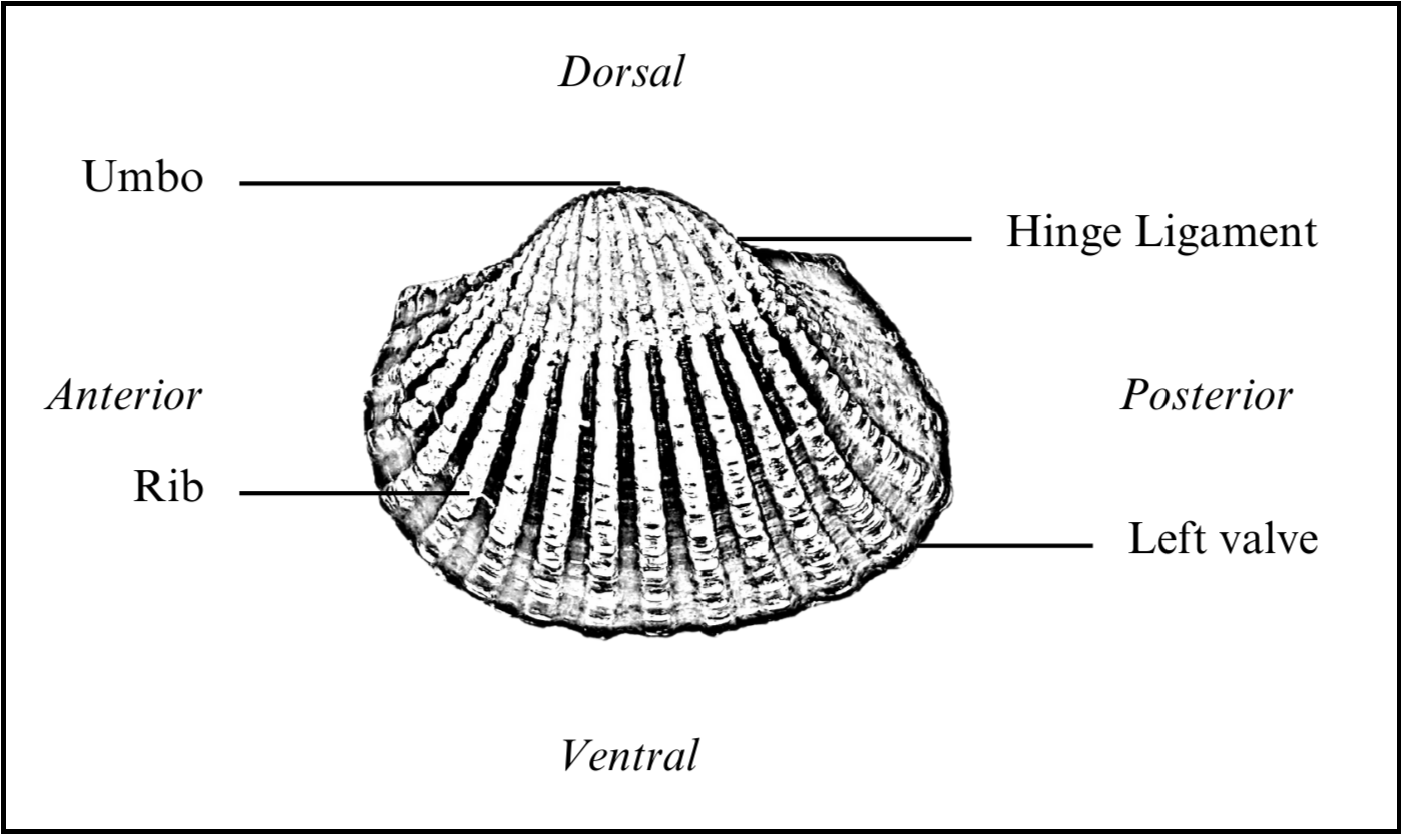
\includegraphics[width=0.9\textwidth]{figures/anatomy.png}
	\caption{Diagram of \Tegillarcagranosa Anatomy}
\end{figure}

\textit{\Tgranosa} shell is medium-sized, fairly thick, ovate, and convex with both valves being equal in size but asymmetrical from the hinge. The top edge of the dorsal margin is straight while the front is rounded and slopes downward with its back being obliquely rounded with a concave bottom edge. It has a narrow diamond-shaped ligament near the hinge with 3-4 dark chevron markings although some may be incomplete. The shell’s outer layer or the periostracum is smooth and brown with a straight hinge line and 40-68 fine short teeth arranged in a straight line. The beak or the prosogyrate curves forward with the shell having 18-21 raised ribs with blunt nodules, having spaces between them. The inner shell is white with crenulations along the valves' ventral, anterior, and posterior margins. The posterior adductor scar is elongated and squarish while the anterior adductor scar is similar but smaller in size. The mantle covering the bulk of \textit{T. granosa’s} visceral mass is thin but the edges are thick and muscular. It bears the impression of the crenulated shell edges. Their foot is large with a ventral grove with no byssus or thread-like attachment. The  \textit{T. granosa’s} soft body is blood red \cite{narasimham1988}.  

\Tgranosa is one of the most well-known marine bivalves given that they are a protein-rich food, known for their rich flavor, substantial nutritional benefits, a good source of vitamins, low in fat, and contains a considerable amount of iron, important in combating anemia \cite{zha2022}. Blood cockles were collected by locals inhabiting the brackish mudflats during the low tides for consumption and sold in the market as a source of livelihood \cite{miranda2023}. \Tgranosa is not only valuable for its market and food purposes, but also facilitates an important role in marine ecosystems as a food source for various organisms like wading birds, intertidal-feeding fish, and crustaceans such as shore crabs and shrimps \cite{burdon2014}. Blood cockles can act as sentinel species and a bioindicator of marine pollutants such as heavy metals \cite{ishak2016} and polycyclic aromatic hydrocarbons (PAHs) \cite{sany2014}. Additionally, cockle shells can be utilized to create a cost-effective catalyst for biodiesel production by providing calcium oxide \cite{boey2011waste}.

Determining the sex of bivalves is important for three reasons namely: diversity, environmental benefits, and economic significance \cite{breton2010novel}. Firstly, with the estimated 25, 000 living species under class Bivalvia, it would be a suitable resource to develop a broader understanding of their evolution of the sex and sex determination mechanism  \cite{breton2010novel}. Second, studying sex determination is important since bivalves are utilized as bioindicators of environmental health. This would pave the way for understanding bivalves' life cycle and population dynamics in determining different factors that affect them \cite{campos2012}. Thirdly, the immediate and practical reason to unveil the sex determination mechanism is the economic and nutritional importance of bivalves as a large population of people rely on fish and shellfish as sources of food and nutrition \cite{naylor2000}. Additionally, male and female aquaculture commodities have different growth and economic values. Male Nile tilapia, for example, grow faster and have lower feed conversion rates than females, female Kuruma prawns (\textit{Penaeus japonicus}) are generally larger than males at the time of harvest \cite{budd}. 

Clearly, much more work is required to understand the mechanisms underlying sexual dimorphism in bivalves, specifically \textit{T. granosa}. Just like the other aquaculture commodities, sex affects not just reproduction but it can affect market preference, and underlying economic value, making the determination of sex important for meeting consumer demands. These are the increasing significance of the \Tgranosa despite the lack of reviewed articles in the Philippines.

\section{Current Methods of Sex Identification in \Tegillarcagranosa}

The current sex identification methods in \Tegillarcagranosa range from invasive histological techniques to less invasive methodologies like temperature-induced spawning. Each approach comes with its pros and cons regarding accuracy, feasibility, and impact on natural populations.
Induced spawning and larval rearing are considered as the less invasive techniques used to study \textit{Tegillarca granosa}. In the Philippines, limited research has been done on the \Tegillarcagranosa (Linnaeus, 1758), and this study, titled Initial Attempts on Spawning and Larval Rearing of the Blood Cockle, \Tegillarcagranosa in the Philippines, is conducted by Denise Vergara Miranda and Victor Marco Emmanuel Nuestro Ferriols (2023). The researchers conducted experiments on induced spawning and larval rearing, discovering that the eggs of female \Tgranosa were salmon pink, while the sperm released by males looked milky. After spawning, the researchers successfully generated 6, 531, 000 fertilized eggs.

They highlighted the importance of \Tgranosa and other anadarinids as a food source that was established worldwide, especially in Malaysia and Korea. However, in the Philippines, the bivalve aquaculture of the clam species is still limited. The experiment which focuses on the culture and rearing of \Tgranosa was attempted by subjecting the wild broodstocks to a series of temperature fluctuations to induce the spawning of gametes. This is currently the most natural and least invasive method for bivalves \cite{aji}. The study of Miranda and Ferriols aimed to pave the way to the sustainable production of \Tgranosa seeds for aquaculture production and stock enhancement despite the scarcity of documented hatchery culture of \Tgranosa from larvae to adults that is available in the Philippines.

In the study entitled, The earliest example of sexual dimorphism in bivalves — evidence from the astartid Nicaniella (Lower Jurassic, southern Germany), the researchers utilized Principal Component Analysis and Fourier Analysis as a non-invasive method that investigates sexual expression in the \textit{Nicaniella rakoveci}. In the study, researchers discovered that the bivalves with crenulations were found to have a different shell shape, which made them more inflated than those without crenulations. This suggests that when they became females, they adapted to hold more eggs, rather than for protection from predators as previously thought. The formation of crenulations is likely part of the genetic process that controls both the sex change and the changes in shell structure \cite{karapunar2021}. Overall, the findings demonstrate that the genetic mechanisms for sex change and shell morphology in bivalves existed as early as the Early Jurassic, contributing to our understanding of bivalve diversity and evolution. Thus, the researchers concluded that crenulations serve as a morphological marker for identifying the sex and reproductive stage of these bivalves  \cite{karapunar2021}.

On the other hand, invasive techniques such as histological analysis offer a more thorough but harmful method for determining the sex of \textit{T. granosa}. A study on the Spawning Period of Blood Cockle \Tegillarcagranosa (Linnaeus, 1758) in Myeik Coastal. 240 blood cockle samples were examined for sex and gonad maturity stages using histological examination, with shell lengths ranging from 26-35mm and shell weights from 8.1-33g. For histological analysis, the whole soft tissues were removed from the shell and the flesh containing most parts of the gonads was fixed in formalin, dehydrated in an upgraded series of ethanol, and cleared in xylene. This invasive method allows for precise identification of the gonadal maturation stages based on the cellular and structural changes in the gonads.

The classification of the gonad stages used was by Yurimoto et al. (2014). There are five maturation stages of gonadal development: immature (Stage I), developing (Stage II), mature (Stage III), spawning (Stage IV), and spent (Stage V) stages. The sex of the \Tgranosa was confirmed by the color of the gonad and by conducting a histological examination of the gonads. During the immature stage, sex determination was indistinguishable due to the difficulties of observing the germ cells. In the developing stage, the spermatocytes and a few spermatids can be seen for males, and immature oocytes are attached to the tube wall for the female. In the mature stage, the follicles are full of spermatozoa with their tails pointing towards the center of the tube for the male and the female are full of mature oocytes that are irregular or polygonal in shape with the oval nucleus. Upon reaching spawning, some spermatozoa are released, causing the empty space in the follicle wall for males and females there is a decrease in the number of mature oocytes and it exhibits nuclear disappearance due to the breakdown of the germinal vesicle. Lastly, the spent stage is where the genital tube is deformed and devoid of spermatocytes which have completely spawned. In the female, the genital tube is deformed and degenerated making it empty. The morphology of the cockle gonad shows that the area of the gonad increases according to the increased levels of gonad maturity. The coloration of the gonad tissue layer in the blood cockle varies from orange-red to pale orange in females and from white to grayish-white in males for different maturity stages \cite{may2021}. 

Although the histological examination is the most reliable method for obtaining accurate information on the reproductive biology and sex determination of \textit{T. granosa}, it has limitations. Given its invasive nature, this approach requires the dissection and destruction of specimens, making it unsuitable for continuous monitoring and conservation efforts. Moreover, the current understanding of sex determination in bivalves and mollusks is poor, and no chromosomes that can be differentiated based on their morphology have been discovered \cite{afiati2007}. There exists a study that can provide insight into the sex-determining factor in bivalves but  \textit{N. schoberti} is more difficult to analyze concerning potential sexual dimorphism. Thickening the edges of the shell increases its inflation, which means the shell can hold more space inside. This extra space helps protandrous females accommodate more eggs.

\section{Machine Learning and Deep Learning in Biological Studies}
Machine learning has the potential to improve the quality of life of human beings and has a wide range of applications in terms of research and development. The term machine learning refers to the invention and algorithm evaluation that enables pattern recognition, classification, and prediction based on models generated from available data \cite{tarca2007}. The study of machine learning methods has advanced in the last several years including biological studies. In biological studies, machine learning has been used for discovery and prediction. This section will explore existing machine learning studies that are applied in biological sciences highlighting the identification of sex in shells, bivalves, and mollusks.

\subsection{Deep Learning for Phenotype Classification in Ark Shells}
In the study, the researchers utilized three (3) convolutional neural network (CNN) models: the Visual Geometry Group Network (VGGnet), the Inception Residual Network (ResNet), and the SqueezeNet \cite{kim2024}. These deep learning models are utilized to the ark shells namely \textit{Anadara kagoshimensis}, \textit{Tegillarca granosa}, and \textit{Anadara broughtonii} to identify the phenotype classification. 

The researchers classified the ark shells based on radial rib count where they investigated the difference in the number of radial ribs between three species and were counted. Their CNN-based model that classifies images of three ark shells can provide a theoretical basis for bivalve classification and enable the tracking of the entire production process of ark shells from catching to selling with the support of big data, which is useful for improving food safety, production efficiency, and economic benefits \cite{kim2024}.

\subsection{Geometric Morphometrics and Machine Learning for Species Delimitation}
In \textit{Geometric morphometrics and machine learning challenge currently accepted species limits of the land snail Placostylus (Pulmonata: Bothriembryontidae) on the Isle of Pines, New Caledonia}, the shell size was quantified using centroid size from the Procrustes analysis, and both the shape and size information were used in training the machine learning model. Their study concluded that the researchers support utilizing both methods: supervised and unsupervised machine learning, rather than choosing either of them individually. In general, their research contributes to the growing number of studies that have combined geometric morphometrics, with the aid of machine learning which is helpful in biological innovation and breakthrough \cite{quenu2020}.

\subsection{Contour Analysis in Mollusc Shells Using Machine Learning}
Tuset et al., (2020) in their study, \textit{Recognising mollusc shell contours with enlarged spines: Wavelet vs Elliptic Fourier analyses}, mentioned Gastropod shells have large spines and sharp shapes which differ based on environmental, taxonomic, and evolutionary influences. The researchers stated that classic morphometric methods may not accurately depict morphological features of the shell, especially when using the angular decomposition of the contour. The current research examined and compared the robustness of the contour analysis using wavelet transformed and Elliptic Fourier descriptors for gastropod shells with enlarged spines. For that, the researchers analyzed two geographical and ecologically separated populations of \textit{Bolinus brandaris} from the NW Mediterranean Sea. Results showed that contour analysis of gastropod shells with enlarged spines can be analyzed using both methodologies, but the wavelet analysis provided better local discrimination. From an ecological perspective, shells with various sizes of spines in both areas indicate a broad adaptability of the species.

\subsection{Machine Learning for Shape Analysis of Marine Organisms}
In the study of Lishchenko and Jones (2021), titled \textit{Application of Shape Analyses to Recording Structures of Marine Organisms for Stock Discrimination and Taxonomic Purposes}, they utilized geometric morphometrics (GM) as an approach to the traditional method of collecting linear measurements with the application of multivariate statistical methods and outline analysis in recording the structures of marine organisms. The main taxonomic categories (mollusks, teleost fish, and elasmobranchs) with their hard bodies have been used as an indication of age and a determinable time-scale and structure continue to go through life \cite{arkhipkin2005, kerr2014}. This study has explored variations in the morphometry of recording structures in stock discrimination and systematics. The researchers utilized the principal component analysis rather than the traditional approach, which helps simplify the data without losing important information. They utilized landmark-based geometric morphometrics which has three different types namely: discrete juxtaposition of tissue, maxima or curvature or other morphogenetic processes, and lastly, the extremal points are constructed landmarks.

Generalized Procrustes Analysis (GPA) is a common superimposition technique in landmark-based geometric morphometrics that aligns landmarks via translation, scaling, and rotation to eliminate non-shape deviations \cite{zelditch2004}. However, there is a limit to the amount of smooth areas that may be captured, and it is possible to overlook significant shape details. Utilization of the semi-landmarks enhanced the shape description \cite{adams2004}. The researchers observed that using an outline-based approach would be more effective than using a landmark-based approach.

Another approach is the Fourier analysis which is a curve-fitting approach commonly used due to its well-known mathematical background and how general functions can be decomposed into trigonometric or exponential functions with definite frequencies. It has two main approaches namely: Polar Transform (PT) in which it expresses the outline using equally spaced radii and Elliptical Fourier Analysis (EFA) which separately analyzes the x and y coordinates of the shape. The PT works for simple rounded outlines and has the tendency to miss details in more complex shapes, unlike EFA which can handle complex, convoluted outlines \cite{zahn1972, doering1990, ponton2006}. Many researchers view EFA as the most effective Fourier method for providing a comprehensive and detailed description of recording structures \cite{merigot2007, ferguson2011, legua2013, mahe2016}.

Landmark-based methods used in the study showed that there are detectable differences between male and female octopuses. However, the accuracy of determining sex based on these differences was low, similar to the results obtained with traditional morphometric techniques. The study involved a relatively small sample size of 160 individuals, and the structure being analyzed (the stylet, or internalized shell) varies significantly between individuals. Although the results aligned with findings from other studies that attempted to identify gender differences in cephalopods, the researchers concluded that the approach might not be accurate enough for reliable sex determination.

\subsection{Deep Learning for Landmark-Free Morphological Feature Extraction}
In another study, \textit{a deep learning approach for morphological feature extraction based on variational auto-encoder: an application to mandible shape}, the Morpho-VAE machine learning approach was used to conduct a landmark-free shape analysis. Morpho-Vae reduces dimensions by concentrating on morphological features that distinguish data with different labels using an image-based deep learning framework that combines unsupervised and supervised machine learning. After utilizing the method in primate mandible images, the morphological features reveal the characteristics to which family they belonged. Based on the result, the method applied provides a versatile and promising tool for evaluating a wide range of image data of biological shapes including those missing segments.

\subsection{Machine Learning for Sex Differentiation in Abalone}
In the study, \textit{Towards Abalone Differentiation Through Machine Learning}, researchers identified a problem in abalone farming which is having to identify the sex of abalone to apply measures for its growth or preservation. The researchers classified abalone sex using machine learning. Researchers trained the machine to classify different types of classes which are male, female, and immature. Based on the result, demonstrated the impact of utilizing linear classifiers. 

Similarly, in the study, \textit{Data scaling performance on various machine learning algorithms to identify abalone sex}, the researchers of the University of India (2022), focused on the data scaling performance of various machine learning algorithms to identify the abalone sex, specifically using min-max normalization and zero-mean standardization. The different machine learning algorithms are the Supervised Vector Machine (SVM), Random Forest, Naive Bayesian, and Decision Tree. Their study aims to utilize machine learning in terms of identifying the trends and distribution patterns in the abalone dataset. Eight features of the abalone dataset (length, diameter, height, whole weight, shucked weight, viscera weight, shell weight, ring) were used to determine the three sexes of Abalone. Their data has been grouped based on sex which are Female, Male, and Infant. They utilized the Synthetic Minority Oversampling Technique (SMOTE) in data balancing for the preprocessing of the data. Followed by data scaling or normalization where it converts numeric values in a data set to a general scale without distorting differences in the range of values. Then they classified by splitting the data into training and testing sets \cite{arifin2021}. 

The researchers found out that the Naive Bayes performs more consistently than other algorithms when the abalone dataset was applied to both min-max and zero-mean normalization has the highest to lowest average accuracy, respectively 62.37\% (Random Forest), 59.49\% (SVM kernel RBF), 57.20\% (Decision Tree), 56.59\% (SVM linear kernel), and 53.39\% (Naïve Bayesian). Overall, despite the decrease in the performance with the normalization, the Random Forest achieves the highest average balanced accuracy of 74.87\%, sensitivity of 66.43\%, and specificity of 83.31\%. Liu et al. found that Random Forest not only can handle large and complex datasets and can run in parallel using multiple random forests but is also more accurate than other algorithms because it selects the best features to improve model performance \cite{arifin2021}. 

\subsection{Machine Learning for Geographical Traceability in Bivalves}
In the study, \textit{BivalveNet: A hybrid deep neural network for common cockle (Cerastoderma edule) geographical traceability based on shell image analysis}, the researchers incorporated computer vision and machine learning technologies for an efficient determination of blood cockle harvesting origin based on the shell geometric and morphometric analysis. It aims to improve the traceability methodologies in these organisms and its potential as a reliable traceability tool. Thirty \textit{Cerastoderma edule} samples were collected along the five locations on the Atlantic West and South Portuguese coast with individual images processed using lazy snapping segmentation, spectro-textural-morphological phenotype extraction, and feature selection through hybrid Principal Component Analysis and Neighborhood Component Analysis \cite{concepcion2023}. 

The researchers developed a non-invasive image-based traceability technique, an alternative to the chemical and biochemical analysis of the bivalves. It was able to incorporate machine learning methods to promote lesser human intervention The researchers discovered that BivalveNet emerged as the superior model for bivalves with 96.91\% accuracy which is comparable to the accuracy of the destructive methods with 97\% and 97.2\% accuracy rate. The result of the study aided the researchers in concluding that there is a possibility of on-site evaluation of the bivalve through the implementation of a mobile app would allow the public and official entities to obtain information regarding the provenance of seafood products’ traceability because of its non-invasive and image-based aspects \cite{concepcion2023}.


\Tegillarcagranosa is known for having no sexual dimorphism. However, through several related studies, the researchers can apply how family shells of \Tegillarcagranosa have been identified based on its morphological and morphometric characteristics, and the methods used in machine learning in identifying its sex. 

\section{Limitations on Sex Identification in \Tegillarcagranosa}
To date, no distinction has been made between the male and female \Tgranosa in sexing methodology. In cockle aquaculture without clearly apparent sexual dimorphism, sexing can be performed using invasive methods such as chemical stimulation, dissection, and gonad-stripping. Induced spawning, specifically temperature shocking, is the most natural and least invasive method for bivalves \cite{aji}. However, the method \cite{wong2018} of immersing cockles in water from hot to cold with a specific temperature requires deliberate and careful manipulation of the temperature over a specific period and would require constant management and monitoring.

Recent studies involved non-invasive methods, with a specific emphasis on morphological characteristics as indicators of sex differentiation. However,  Tatsuya Yurimoto et al. (2014) stated that the existing methods for determining the sex of bivalves and mollusks in general are somewhat limited \cite{afiati2007}. At present, there is no recorded evidence of sexual dimorphism in \textit{Tegillarca granosa}. Gonochoristic is the classification given to \Tegillarcagranosa \cite{lee1997}. However, Lee et al. (2012) reported that the sex ratio varied with shell length, suggesting that sex might alter. 

Hermaphrodites can exhibit either sequential (asynchronous) or simultaneous (synchronous or functional) characteristics. Sequential hermaphrodites switch genders after being male or female for one or multiple yearly cycles. \cite{heller1993, gosling2004, collin2013}. Sex change and consecutive hermaphroditism have been observed in different bivalve species, including Ostreidae, Pectinidae, Veneridae, and Patellidae. However, macroscopically differentiating bivalve sex is challenging. The only way it may be identified is through histological analysis of gonad remains but to do so there is an act of killing the organism \cite{coe1943, gosling2004}. Verification of sex change in bivalves to classify whether male or female while they are alive is challenging since they need to be re-confirmed and re-evaluated to be the same individual after a year.

Lee et al. (2012) found out that \textit{T. granosa}, a species in Arcidae, has been discovered to be a sequential hermaphrodite, with the sex ratio changing with an increase in the shell size. In bivalves, sex changes usually happen when the gonad is not differentiated between spawning seasons \cite{thompson1996}. But in \textit{T. granosa}, after the spawning season, sex changes during its inactive phase. Results showed a 15.1\% sex change ratio, with males having a higher sex change ratio (21.2\%) than females (6.2\%). The 1+ year class had a higher ratio (17.8\%) than the 2+ year class (12.1\%). Thus, this study indicates that \Tgranosa is a sequential hermaphrodite. The results of the study demonstrated that the bivalve's age affects the sex ratio and degree of sex change, but additional in-depth investigation is required to determine the role that genetic and environmental factors play in these changes.

No literature in the study of mollusks specifically addresses the machine learning algorithm used to determine the sex of \Tgranosa bivalves in various models. Nevertheless, various techniques such as shape analysis, morphometric analysis, Wavelet, and Fourier analysis, as well as different deep learning models like VGNet, ResNet, and SqueezeNet in CNN networks are utilized for phenotype classification, while different machine learning algorithms could serve as the foundation for this research project

\section{Synthesis of the Study}
This section of the paper summarizes the technologies used in the different studies related to the pursuit of the study entitled, Non-invasive Sex Identification of \Tgranosa using machine learning.

\begin{table}[]
	\centering
	\renewcommand{\arraystretch}{3} 
	\begin{adjustbox}{scale=0.55,center}
	\normalsize
	\begin{tabular}{|p{5cm}|p{5cm}|p{8cm}|p{8cm}|p{8cm}|}
		\hline
		\centering
		\textbf{Author} &
		\centering
		\textbf{Technology / Method Used} &
		\centering
		\textbf{Description of Problem} &
		\centering
		\textbf{Pros} &
		\textbf{Cons} \\ \hline
		
		D. V. Miranda and V. M. E. N. Ferriols &
		Temperature shock &
		No recent studies are available on the production and rearing of \textit{\Tgranosa} in the Philippines. &
		Employed less invasive techniques which minimize the stress in \textit{\Tgranosa} and can lead to better survival rates. &
		Time-consuming as the entire process from fertilization to the spat stage took 120 days. \\ \hline
		
		Karapunar, Baran and Werner, W. and Fürsich, F. T. and Nützel, A. &
		Morphometric analysis, microscope imaging, principal component analysis (PCA), and Fourier shape analysis &
		To address the observed shell dimorphism in the Early Jurassic bivalve \textit{Nicaniella rakoveci}, namely the presence or lack of crenulations on the ventral shell margin, and whether these variations represent sexual dimorphism and sequential hermaphroditism. &
		The methods used reveal significant morphological differences with regard to sexual dimorphism. &
		There could be misinterpretation of the shape differences of bivalves due to the constraints and resolution of technologies used. \\ \hline
		
		K. May and C. Maung and E. Phyu and N. Tun &
		Histological examination &
		The need to understand the reproductive period of \textit{\Tgranosa} in Myeik to ensure sustainable aquaculture and to prevent overexploitation. &
		Method used allows for accurate sex identification based on the histological characteristics and color of the gonads. &
		Invasive technique used to determine the sex of \textit{\Tgranosa} through gonad histological analysis. \\ \hline
		
		E. Kim and S.-M. Yang and J.-E. Cha and D.-H. Jung and H.-Y. Kim &
		Convolutional neural network (CNN) models, VGGNet, Inception-ResNet, SqueezeNet &
		Traditional methods of recognizing and classifying ark shell species based on shell traits are time-consuming and inaccurate. &
		Automated classification of the three ark shells using a deep learning model obtained an accuracy of 92.4\%. &
		Challenges may arise with certain ark shells that share similar morphology. \\ \hline
		
		Mathieu Quenu and S. A. Trewick and F. Brescia and M. Morgan-Richards &
		Neural network analysis (supervised learning) and Gaussian mixture models (unsupervised learning) &
		To determine whether the shape and size of the snail’s shells can distinguish between two \textit{Placostylus} species, particularly in groups that appear to be hybrids. &
		Combining geometric morphometrics and machine learning effectively answers biological issues, providing insights into species classification and possible hybridization. &
		Difficulty classifying intermediate phenotypes, with potential for overfitting and misclassification in both learning methods. \\ \hline
		
		V. M. Tuset and E. Galimany and A. Farrés and E. Marco-Herrero and J. L. Otero-Ferrer and A. Lombarte and M. Ramón &
		Wavelet functions and Elliptic Fourier descriptors &
		Addresses the difficulty of accurately defining phenotypic diversity in gastropod shells. &
		Advanced contour analysis methods allow accurate differentiation of gastropod shell forms. &
		Cannot clarify the causes of phenotypic variation in the two populations studied. \\ \hline
		
		Fedor Lishchenko and Jones, J. B. &
		Landmark- and outline-based Geometric Morphometric methods &
		To address difficulties in differentiating between stocks of marine organisms to prevent misidentification that could affect conservation and management. &
		Shape analysis improves taxonomic classification precision and offers close distinction between related species or organisms. &
		Landmark-based methods can be sensitive to landmark placement. \\ \hline
		
		M. Tsutsumi and N. Saito and D. Koyabu and C. Furusawa &
		Morphological regulated variational AutoEncoder (Morpho-VAE) &
		The need for reliable, landmark-free methods, such as a modified variational autoencoder, to extract and decipher complex shapes from image data. &
		Employs dimension reduction and feature extraction, making it a user-friendly tool for biology non-experts. &
		Limited sample size in certain families presented challenges. \\ \hline
		
		Barrera-Hernandez, R. and Barrera-Soto, V. and Martinez-Rodriguez, J. L. and Ríos-Alvarado, A. B. and Ortiz-Rodríguez, F. &
		Machine learning algorithms &
		Identifying the sex of abalones is challenging for producers applying specific growth or preservation strategies. &
		Machine learning algorithms accurately classify abalone sex into three categories: male, female, and immature. &
		Selected features may not fully capture the complexity of abalone morphology. \\ \hline
		
		Concepcion, R. and Guillermo, M. and Tanner, S. E. and Fonseca, V. and Duarte, B. &
		EfficientNet-Bo, ResNet101, MobileNetV2, InceptionV3 &
		Addresses the difficulty of accurately tracing bivalve harvesting origins using computer vision and machine learning algorithms to enhance seafood traceability and combat food fraud. &
		Non-invasive, image-based tools for bivalve traceability provide faster, cheaper, and equally accurate alternatives to traditional chemical analysis methods. &
		Small sample size (only 30 cockles) limits model reliability. \\ \hline
		
	\end{tabular}
	\end{adjustbox}
\end{table}

\newpage

Recent developments and breakthroughs in machine learning offer hopeful solutions for biological issues. Research findings indicate that various machine learning techniques such as CNNs, geometric morphometrics, and deep learning models. They are deemed to be effective for identifying phenotypes and determining the gender of various aquaculture commodities, such as mollusks and abalones. These techniques provide a starting point for creating new, non-invasive ways to differentiate male and female \textit{T. granosa}, potentially addressing the drawbacks of manual and invasive methods. Thus,  machine learning to examine morphological and morphometric features may streamline the process of sex identification.

Nevertheless, the use of machine learning to determine the sex of \Tgranosa has not been fully explored. It lacks up-to-date and significant related literature on using machine learning to identify sex in \textit{T. granosa}, particularly given the species’ possible sequential hermaphroditism and lack of obvious external sexual distinctions.










